\chapter{IST-Analyse}
In dieser Arbeit wird das Bestellsystem von der Party-Service-Website "jungekueche" betrachtet. Dazu zählen auch das Verwaltungssystem des Auftraggebers und die Verwaltungsseite des Kunden. Zuerst wird das Userinterface aus der Sicht von allen drei Akteuren beschrieben. Danach wird die Funktion des Systems evaluiert.

\section{Beschreibung des User Interface (UI) des Bestellsystems} 

\subsection{Anmeldeformular}
Die Anmeldung und die Registrierung für neue Nutzer befindet sich auf einer gemeinsamen Seite. 
Das Anmeldeformular hat zwei Felder, in denen der Benutzer seinen PIN und seine E-Mail eingeben muss. Neben den Feldern steht ein Hinweis, welcher den Kunden mit den nötigen Informationen versorgt, wie er sich anmelden oder registrieren kann.  


\begin{figure}[h]
	\centering
	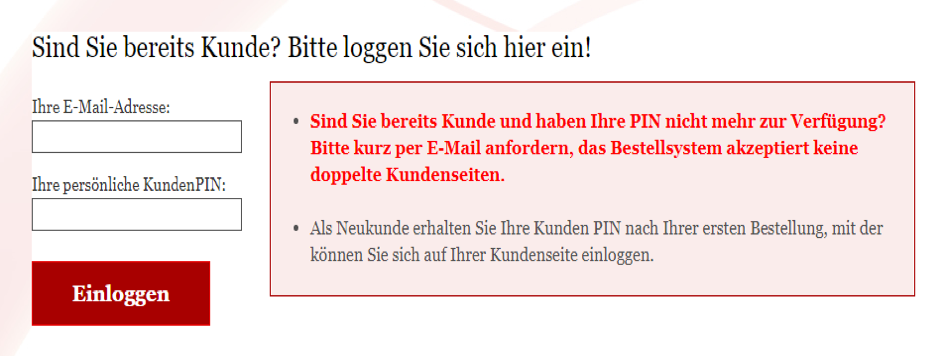
\includegraphics[width=0.7\linewidth]{Graphics/anmeldeformular.png}
	\caption[Anmeldeformular]{Die bisherige Eingabemaske für das Kundenlogin}
	\label{fig:anmeldeformular}
\end{figure}


\subsection{Registerformular}

Falls der Kunde keine PIN hat, muss er sich registrieren. Dieses Formular besteht aus fünf Abschnitten. Im ersten muss der Kunde seine persönlichen Daten angeben. In dem zweiten steht die Informationen des Auftrags. Menü Auswahl ist der nächste Abschnitt. Im vorletzten wird die Zubehörauswahl und Serviceauswahl angezeigt. Der letzte Abschnitt ist die Erklärung zu dem Registrierungsprozess. 

\begin{figure}
	\centering
	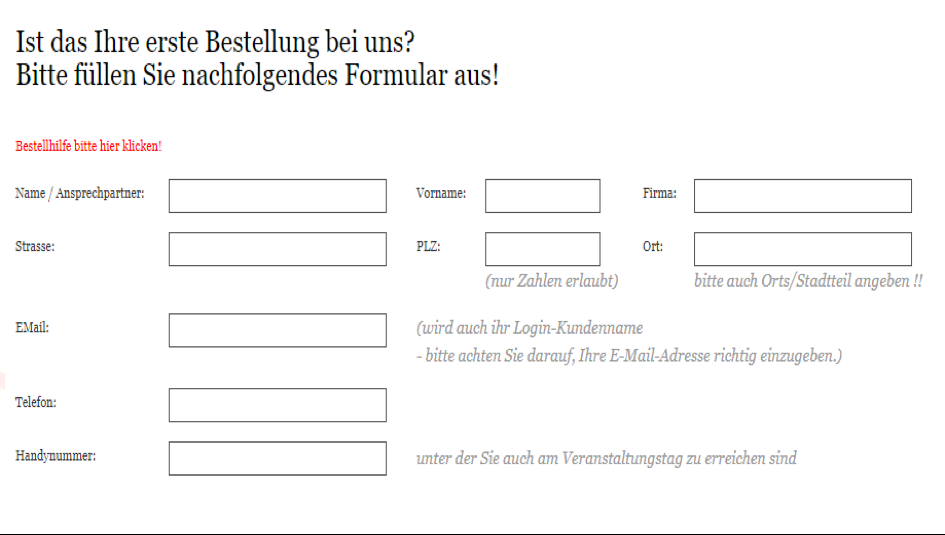
\includegraphics[width=0.7\linewidth]{Graphics/registerForm.png}
	\caption[Registerformular]{Die bisherige Eingabemaske für das Registrierungsformular}
	\label{fig:registerForm}
\end{figure}

\subsection{Auftraggeber - Verwaltung}

Im Fall einer Registeranfrage kann der Auftraggeber sie bestätigen oder löschen. Dem Auftraggeber stehen drei Optionen zur Verfügung; Auftragsverwaltung, E-Mail Verwaltung und Umsatzverwaltung. Zuerst betrachtet man die Auftragsverwaltung. Dort befinden sich 11 Optionen, 9 davon leiten zu eigenen Unteroptionen weiter. Die anderen Zwei sind Speichern und "Abmelden". Durch diese Optionen kann der Auftraggeber die Kundedaten einsehen, editieren, bearbeiten und löschen. Außerdem kann er die dazugehörigen die Nachrichten lesen und löschen. Auch kann er neue und alte Aufträge einsehen und bearbeiten oder löschen.

\begin{figure}[h]
	\centering
	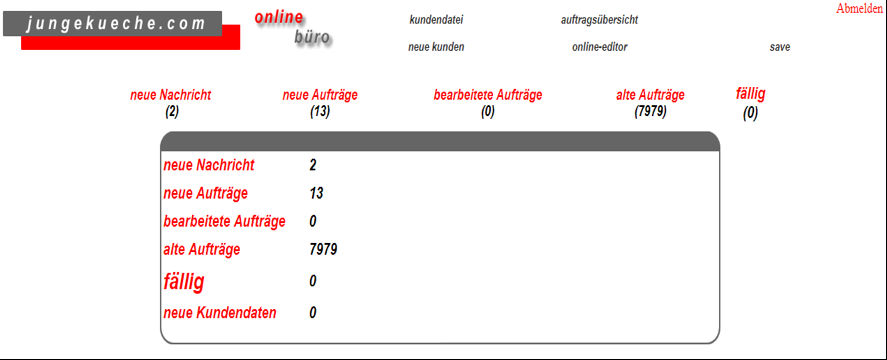
\includegraphics[width=0.7\linewidth]{Graphics/Auftragverwaltung.png}
	\caption[Auftragsverwaltung]{Die bisherige Eingabemaske für die Auftragsverwaltung}
	\label{fig:Auftragverwaltung}
\end{figure}

\subsection{Kundenansicht}

Wenn die Anfrage des Kunden bestätigt wird, bekommt der Kunde einen PIN pe E-Mail. Mit diesem PIN und seiner E-Mail kann der Kunde sich bei "Jungekueche" anmelden. Nach dem Login-Prozess, findet er sich auf einer persönlichen Nutzerseite wieder. Dort hat er eine Übersicht über seine aktuellen und alten Bestellungen, ein Kontaktfenster, in dem er die Nachrichten einsehen oder schreiben kann, sowie eine Art Newsletter. Außerdem gibt es eine Option, durch die der Kunde neue Bestellungen aufgeben kann.  

\begin{figure}[h]
	\centering
	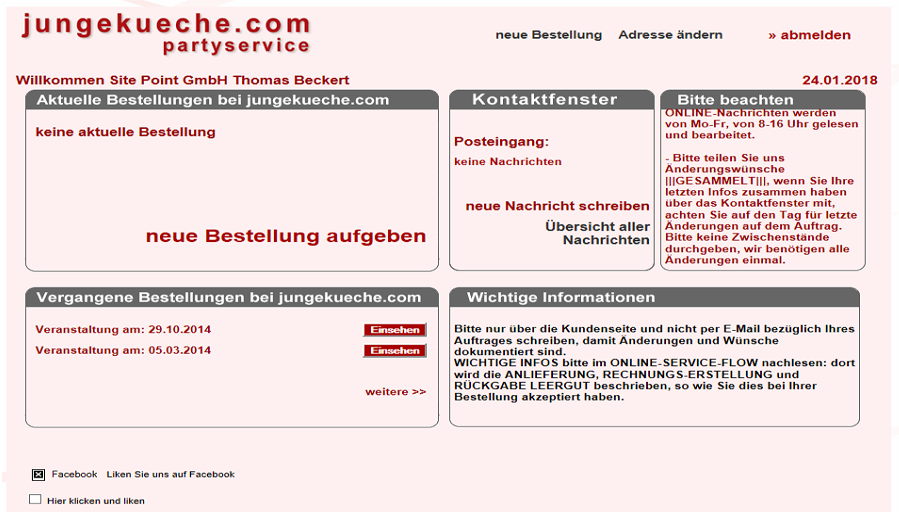
\includegraphics[width=0.7\linewidth]{Graphics/KundenAnsicht.png}
	\caption[Kundeansicht]{Die bisherige Eingabemaske für die Auftragsverwaltung}
	\label{fig:KundenAnsicht}
\end{figure}

\section{Beschreibung der Funktionalität}   

Einer Anmeldung muss immer eine Registrierung vorausgehen. Diese Funktionalität wird mit ASP und ASP.NET realisiert. Die verwendeten Hilfsprogramme sind JQuery, JavaScript, AJAX, HTML und CSS. 

Zuerst wird betrachtet, wie die Kommunikation zwischen den verschiedenen Technologien funktioniert. Das ganze Programm besteht aus Front- und Backend. Das Frontend bezeichnet den Teil des Programms, welches der Nutzer verwendet. Im Backend werden die Daten verarbeitet. Die Verbindung zwischen den beiden wird über JavaScript und JQuery realisiert. Wenn der Benutzer eine Tätigkeit ausführt, werden die eingegebenen Daten über JavaScript Methoden zu dem Backend weitergeleitet. Dort werden sie verarbeitet und über JavaScript Methode aufgerufen. Dort werden sie bearbeitet und wieder zu dem Frontend zugeschickt. Das Backend entsteht aus ASP-Funktionen, in denen sich verschiedenen Methoden befinden, sowie Datenbanken. In den Datenbanken werden die eingegebenen Daten gespeichert.

Abbildung (neue Diagramm.. die Kommunikation zwischen Front- und Backend bzw. Client -Server)

Nach der grundlegenden Kommunikation zwischen Front- und Backend, wird erläutert wie die einzelnen Kommunikationsabläufe zwischen Front- und Backend koordiniert werden.

\subsection{Anmelde- und Registerformular} 

\textbf{Hier wurde noch nicht korrigiert}

Es wird mit dem Bestellseite angefangen, bzw. Anmeldeformular. Wenn die Kunde "Anmeldung" drückt, wird eine HTML Post-Methode aktiviert.  So werden JavaScript- und ASP- Methoden aufgerufen. Die JavaScript-Methoden werden benutzt, damit die Eingabe geprüft wird, ob sie korrekt ist, und ASP-Methoden werden dann aufgerufen. 

Der Registerformular funktioniert auf demselben Prinzip. Wenn die Eingaben eingegeben sind, werden sie geprüft, ob alles korrekt ist, falls alles in Ordnung ist, werden die Eingaben zu dem zugeordneten Daten, bzw. Methoden zugeschickt.

mehr im Anhang - Funktionen

\begin{figure}[h]
	\centering
	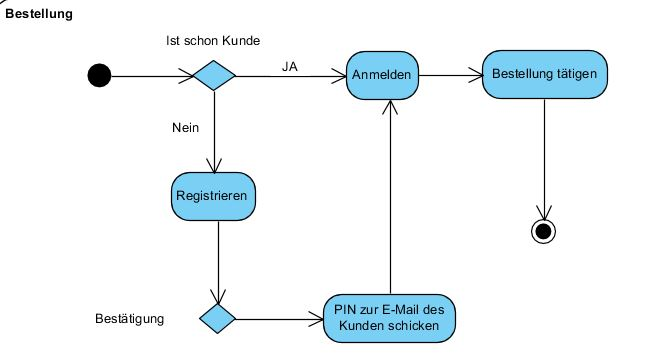
\includegraphics[width=0.9\linewidth]{Graphics/Bestellung.JPG}
	\caption[Anmeldung/Bestellung]{Die bisherige Eingabemaske für den Vorgang der Bestellung/Registrierung}
	\label{fig:Bestellung}
\end{figure}

\subsection{Auftraggeber-Verwaltung}

Hier wird man sich nur mit dem Auftragsverwaltung beschäftigen. Die Auftragsverwaltung, wie es schon beschrieben wurde, besteht auf verschiedenen Optionen. Jetzt lässt sich jeweiliges betrachten, wie es funktioniert. 
	
\subsubsection{Nachricht-Sektion} ermöglicht dem Auftraggeber die Information zu lesen oder löschen. Nach zugeordnetem Wahl wird die Information in der Datenbank "komentar" entweder aufgerufen oder entfernt. 

\begin{figure}[h]
	\centering
	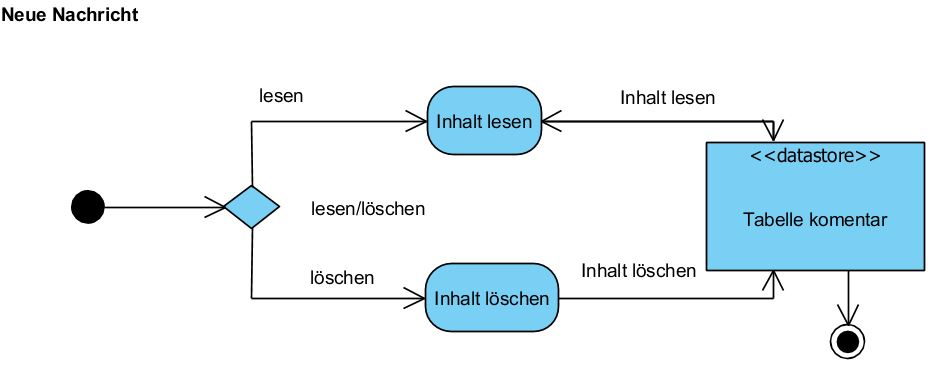
\includegraphics[width=0.8\linewidth]{Graphics/NeueNachricht.JPG}
	\caption[Kommunikation]{Die bisherige Eingabemaske für den Nachrichten lesen oder löschen}
	\label{fig:Kommunikation}
\end{figure}



\subsubsection{Aufträge: Neue, alte und bearbeitende}

Die Funktionalität von allen drei ist dieselbe. Deswegen es wird allgemein erklärt. Der Auftraggeber kann den Auftrag sehen, editieren oder löschen. Alle von diese Aktivitäten ist mit mehrere Datenbanken verbunden, die verschiedenen Informationen über die gewählten Artikel haben. In den Abbildungen \ref{fig:Autrag_Loeschen} und \ref{fig:auftragEinsehen} betrachtet man die jeweilige Funktionalität.


\begin{figure}[h]
	\centering
	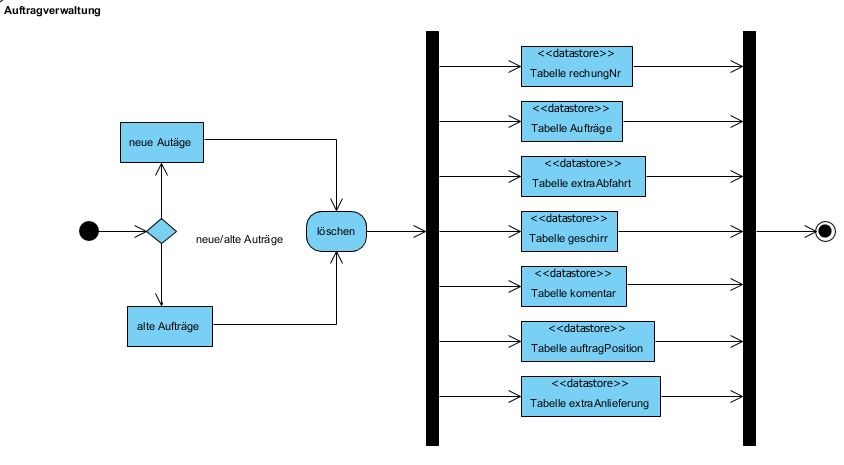
\includegraphics[width=1\linewidth]{Graphics/Autrag_Loeschen.JPG}
	\caption[AutragLoeschen]{Die bisherige Eingabemaske für den Nachrichten lesen oder löschen}
	\label{fig:Autrag_Loeschen}
\end{figure}
 
\begin{figure}[h] 
	\centering
	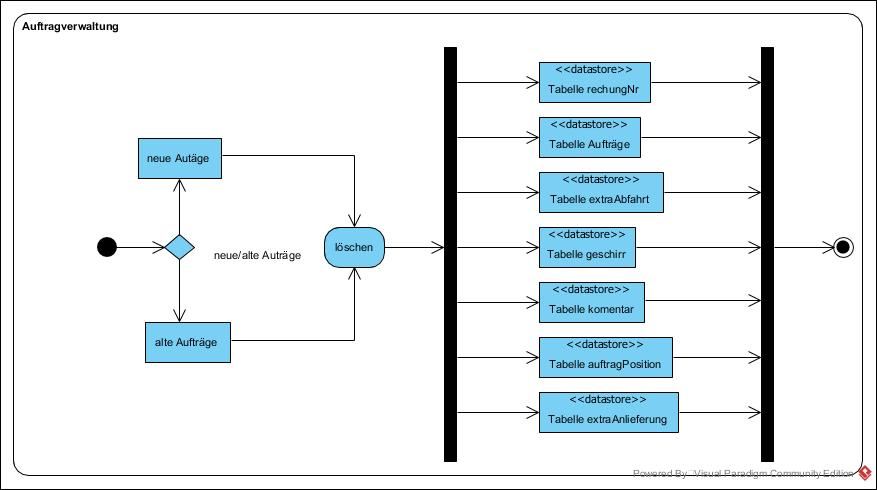
\includegraphics[width=1\linewidth]{Graphics/Auftragverwaltung.jpg}
	\caption[auftragEinsehen]{Die bisherige Eingabemaske für den Nachrichten lesen oder löschen}
	\label{fig:auftragEinsehen}
\end{figure}

\pagebreak
\subsubsection{Kundendatei}

Hier befindet sich die Information über die Kunden. Da kann man die Information editieren oder löschen. Um der bestimmten Kunde schneller zu finden, steht eine Suchmaschine zur Verfügung. Eine bessere Übersicht wird in der Abbildung \ref{fig:KundenDatei} dargestellt. 

\begin{figure}[h]
	\centering
	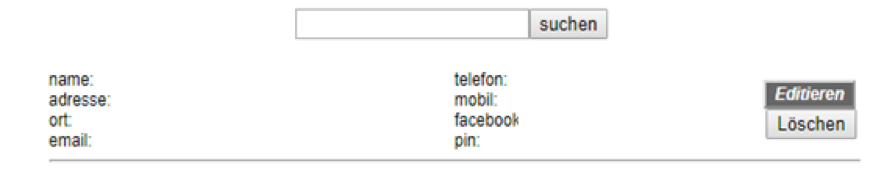
\includegraphics[width=0.7\linewidth]{Graphics/kundenDatei.png}
	\caption[Kundeansicht]{Die bisherige Eingabemaske für die Kundendatei}
	\label{fig:KundenDatei}
\end{figure}

Wenn man editieren oder löschen will, wird es über JavaScript Funktion passiert. Diese Funktion ruft die Methoden auf, die sich in der zugeordneten ASP-Datei befindet. Im "Editor-Fenster" kann man die Daten des Kunden editieren, Login-Daten wie Email an Kunden übermitteln, Wichtige Information für alle Kunden senden, V.I.P-Status des Kunden geben, spezifische Warnungen jeweiligem Kunde aufgeben, Information schreiben, sowie Unterschrift editieren und etc. Besser Verständnis zum diesen Fenster ergibt uns Abbildung \ref{fig:Kunden Editor}


\pagebreak

\begin{figure}[h]
	\centering
	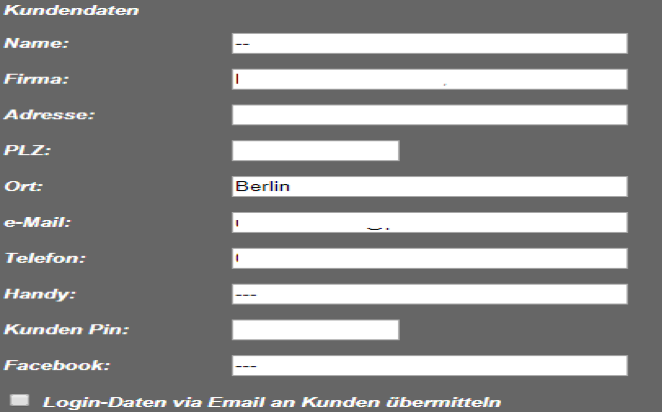
\includegraphics[width=0.7\linewidth]{Graphics/kundeEditieren.png}
	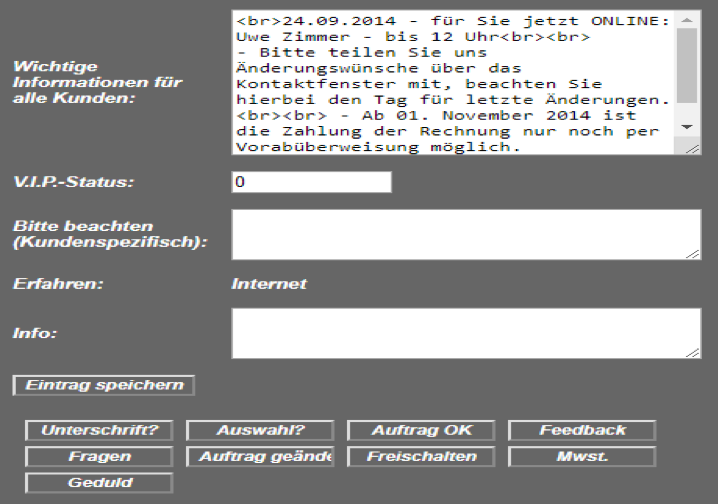
\includegraphics[width=0.7\linewidth]{Graphics/kundeEditieren1.png}
	\caption[Kundeansicht]{Die bisherige Eingabemaske für das Kunden-Editor}
	\label{fig:Kunden Editor}
\end{figure}


Durch JavaScript - Methode wird eine zusätzlichen Möglichkeit zu dem Kunde Nachricht geschrieben. Sie wird aktiviert, wenn der Cursor auf dem bestimmten Kunde, der in der Liste des Adressbuch ist, steht. Die Kommunikation zwischen dem Auftraggeber und dem  Kunde wird auch im Datenbank "komentar" gespeichert. 

Nach allem, was geschrieben ist, soll man sich ein vertieftes Verständnis aufbauen. In folgenden Abbildungen \ref{fig:Kunden Datei Editieren und Löschen} und \ref{fig:Kommunikation Auftraggeber Kunde} kann man sehen, wie genau die Aktivitäten des Auftraggeber passieren und wie funktioniert die Nachricht-Kommunikation.
\pagebreak


\begin{figure}[h]
	\centering
	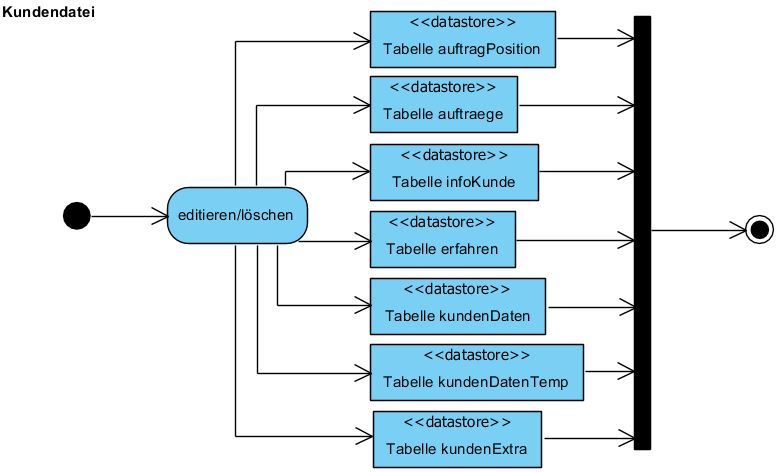
\includegraphics[width=0.7\linewidth]{Graphics/Kundendatei.JPG}
	\caption[Kundeansicht]{Die bisherige Eingabemaske für das Editieren/Löschen Funktion}
	\label{fig:Kunden Datei Editieren und Löschen}
\end{figure}

\begin{figure}[h]
	\centering
	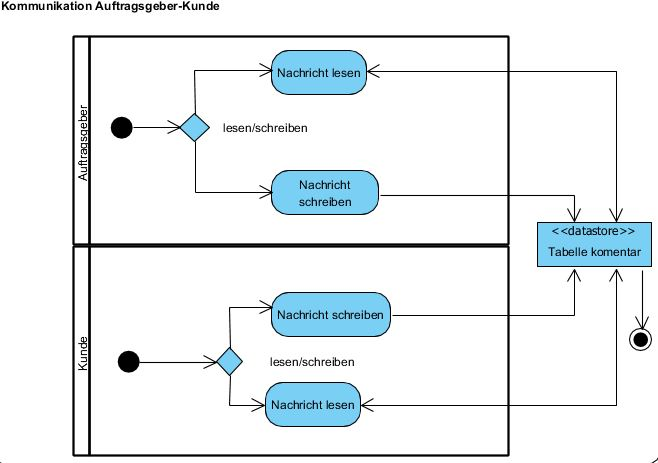
\includegraphics[width=0.7\linewidth]{Graphics/Kommunikation.JPG}
	\caption[Kundeansicht]{Die bisherige Eingabemaske für die Kommunikation zwischen dem Auftragsgeber und dem Kunde}
	\label{fig:Kommunikation Auftraggeber Kunde}
\end{figure}

\subsubsection{Online-Editor}

Durch diese Option kann man die neuen Artikel zu erstellt, editieren und löschen werden können.  Es gibt „Artikel – Arragements“ und „Artikel – Standard“. Wenn schon ein Artikel erstellt wurde, kann er entweder gelöscht, editiert oder zugeordnet werden. 
JavaScript Funktionen werden benutzt, um die Eingabe zu prüfen, ob alles korrekt ist. Wenn alles in Ordnung ist, werden die obengenannten Methoden aus den jeweiligen Dateien aufgerufen. In der folgenden Abbildung \ref{fig: Online-Editor übersicht} ist die Übersicht der Seite zu sehen.
\pagebreak

\begin{figure}[h]
	\centering
	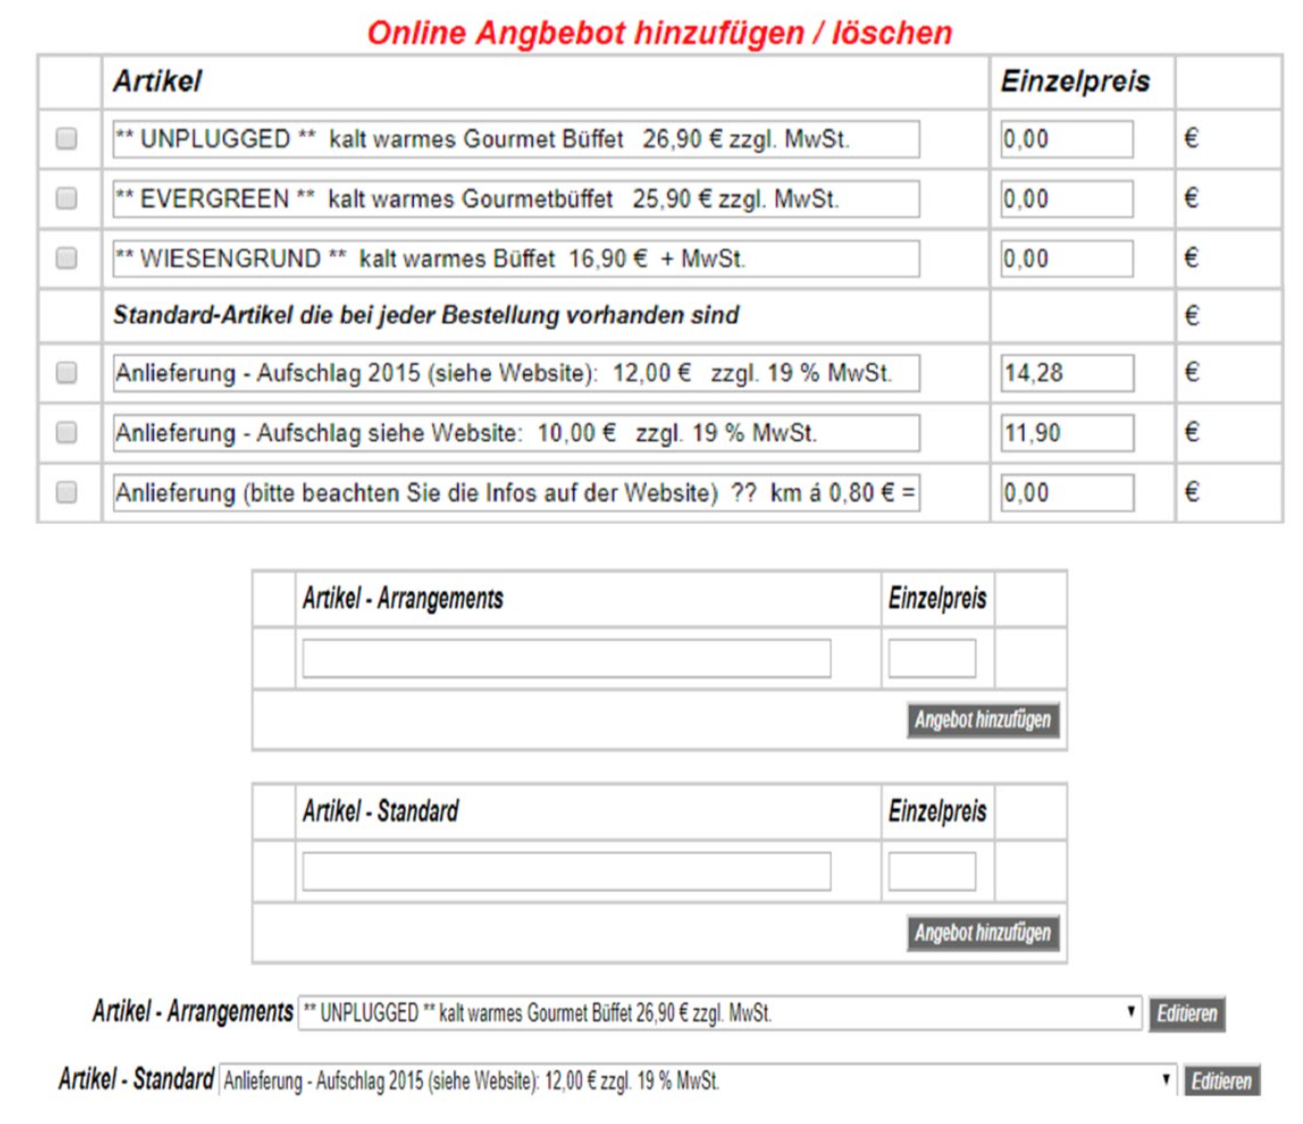
\includegraphics[width=0.7\linewidth]{Graphics/menue-uebesicht.png}
	\caption[Kundeansicht]{Die bisherige Eingabemaske für die Übersicht das Menü}
	\label{fig: Online-Editor übersicht}
\end{figure}

Wenn die Option „Editieren“ zu dem „Artikel-Arrangements“ ausgewählt wird, wird neue Seite geöffnet, in der es vielfältige Möglichkeiten gibt, die Inhalt geändert werden kann. Abbildung \ref{fig: Editor-Menü2}  zeigt uns wie diese Seite aussieht.


\begin{figure}[h]
	\centering
	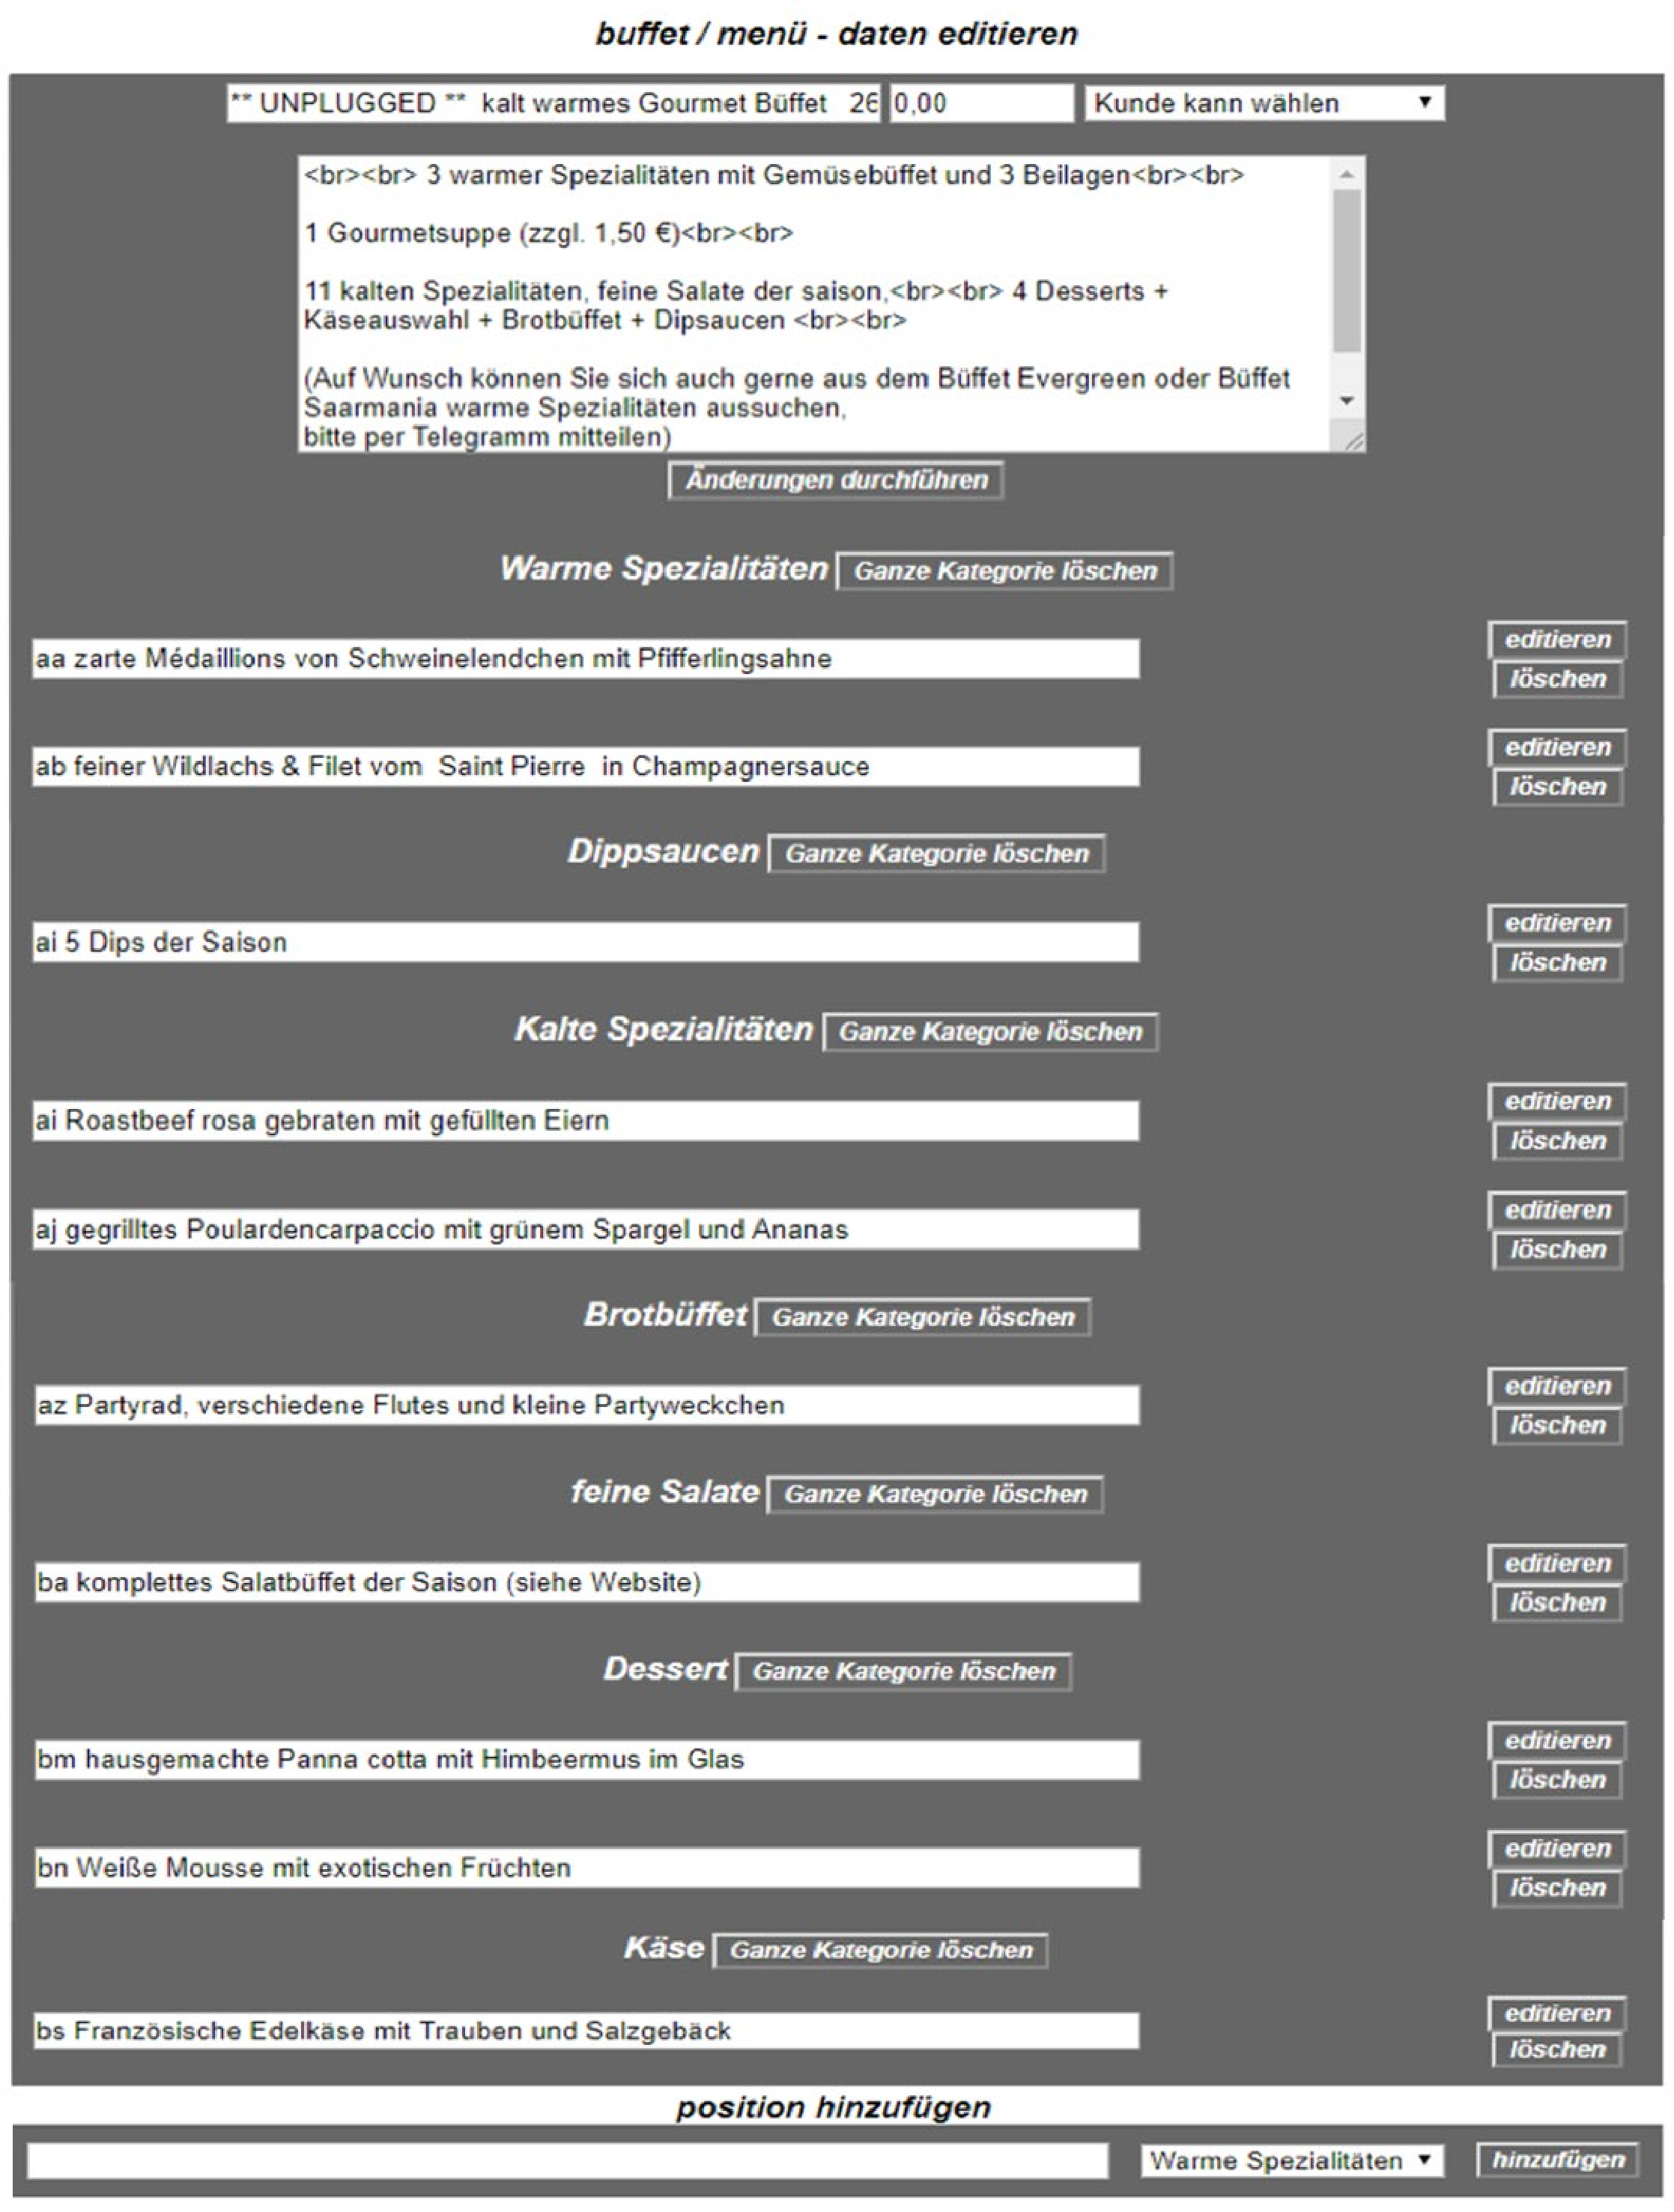
\includegraphics[width=0.7\linewidth]{Graphics/arrangement-Menue-editor.pdf}
		\caption[Kun2deansicht]{Die bisherige Eingabemaske für die Übersicht des Menü-Editor-Arrangements}
	\label{fig: Editor-Menü2}
\end{figure}


Artikel-Standard“ hat nur eine Möglichkeit, editiert zu werden. Sie wird in der Abbildung \ref{fig: Editor-Menü-Standard}   dargestellt.

\begin{figure}[h]
	\centering
	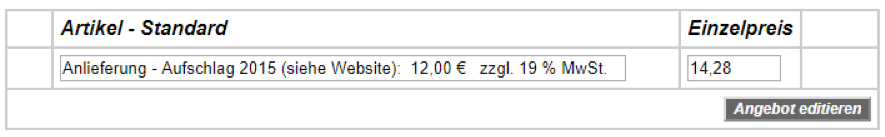
\includegraphics[width=0.7\linewidth]{Graphics/menuStandart.png}
	\caption[Kundeansicht]{Die bisherige Eingabemaske für die Übersicht des Menü-Editor-Standard}
	\label{fig: Editor-Menü-Standard}
\end{figure}

\begin{figure}[h]
	\centering
	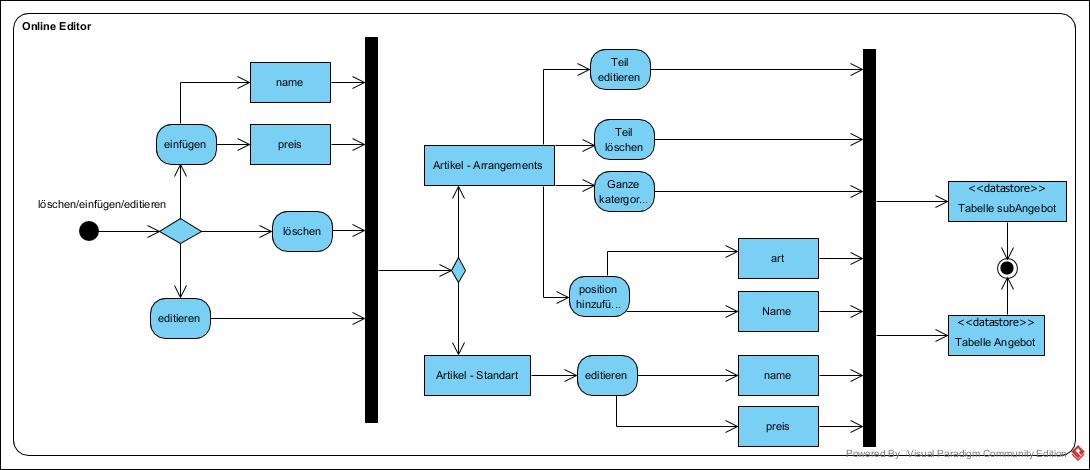
\includegraphics[width=1\linewidth]{Graphics/OnlineEdior.jpg}
	\caption[Kundeansicht]{Die bisherige Eingabemaske für die Funktionalität des Menü-Editor-Standard}
	\label{fig: Editor-Menü-Funktionalität}
\end{figure}
In Abbildung \ref{fig: Editor-Menü-Funktionalität} ist der Zusammenhang zwischen die verschiedenen Funktionen des „Online-Editor“ zu sehen.


\section{Testen} 


Für diese Arbeit wird ein webbasierten Sicherheit-Checker von 1\&1. Nach eine vertiefte Recherche, zeigte sich, dass die Webseite auf eine mittlere Sicherheitsposition steht. Die Webseite ist nach vier Kriterien ohne Beanstandung abgesichert.

\begin{itemize}	
	
\item\ac{SSL} Verschlüsselung – Über SSL wird sichergestellt, dass zwischen User und Server die übertragenen Daten nicht gelesen werden können.

\item Cookies sind auch sicher und so ist der Browser von Dritten über JavaScript unlesbar.

\item Apache-Status ist verboten. Die Status-Seite ist öffentlich nicht erreichbar. So wird den Schutz von potenziellen Angreifern erhöht. 

\item Server Version ist nicht sichtbar. Die Server Version ist öffentlich nicht einsehbar. Damit kann ein Angreifer nicht einfach bekannte Schwachstellen ausnutzen.
\end{itemize}

\begin{figure}[h]
	\centering
	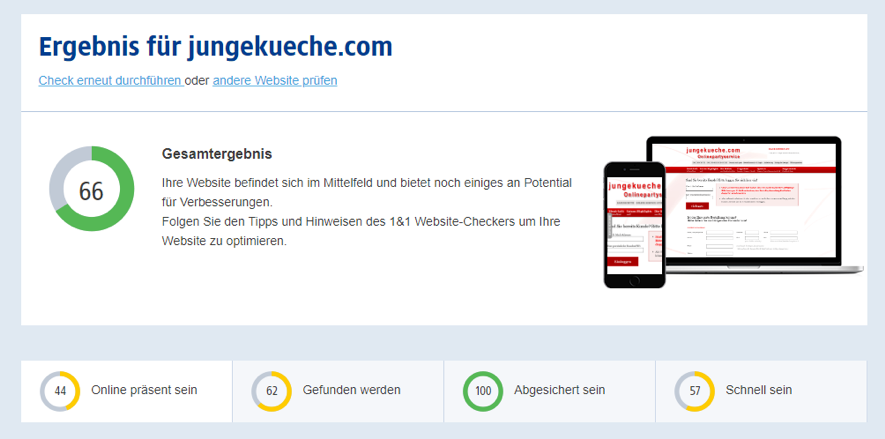
\includegraphics[width=1\linewidth]{Graphics/egebnis1to1.png}
	\caption[Egebniss Von 1zu1]{Ergebnis vom 1zu1}
	\label{fig: Egebniss Von 1zu1}
\end{figure}

Wie man von der Abbildung \ref{fig: Editor-Menü-Funktionalität} sehen kann, ist die Webseite gesichert, aber es gibt einige Bereiche, die eine Optimierung benötigen würde. Sie lädt sich langsam, wird im Browser relativ oft gefunden, aber ist sie gesichert. 

Über noch ein Web-Checker werden die witere Funktionalitäten der Wrbseite analysiert. Observatory\cite[postnote]{bentley:1999} von Mozilla analysiert der Browser im vier Schritten. 

\begin{itemize}	
	\item \ac{HTTP}
	\item \ac{TLS}
	\item \ac{SSH}
	\item \ac{Third-Party Tests}
\end{itemize}

Erste zwei werden betrachtet, weil nur sie wichtig zu dieser Arbeit sind.

\pagebreak

\textbf{HTTP Observatory}

Hier werden aktuelle Sicherheit der Webseite im öffentlichen Internet beobachtet. Alle Anfragen sind über POST- oder GET-Methoden durchgeführt und die Rückmeldungen sind im JSON-Format.
Nach dieser Analyse wird gezeigt, dass \ac{CPS} nicht implementiert wurde. CSP verhindert Weitbereich von \ac{XSS}- und „clickjacking“- Attacken. 
Cookes sind teilweise gesichert. Hier fehlt es „Secure“-Attribut, sowie „SameSite“ und „Prefix“.  Durch „Secure“ werden die Cookies davon abgehalten, dass sie über nicht gesicherten HTTP versendet werden. „SameSite“ hält die Cookies vom \ac{CSRF} Attacken und Cross-Site-Übersendung ab, d. h. es ist möglich, dass es einen Hacker-Angriff auf Computersystem des Benutzers durchgeführt werden \cite[postnote]{bentley:1999}
. Es wird keine \_Host- und \_Secure-Prefixes auf den Namen der Cookies verwendet. Das bedeutet, dass sie nicht gegen Überschreiben geschützt sind. Man kann in der Abbildung \ref{fig: HTTP Observatory: Ergebnis} die genaue Bewertung von der Webseite.
 stellt das Resultat von der durchgeführten Analyse dar.
 
\begin{figure}[h]
	\centering
	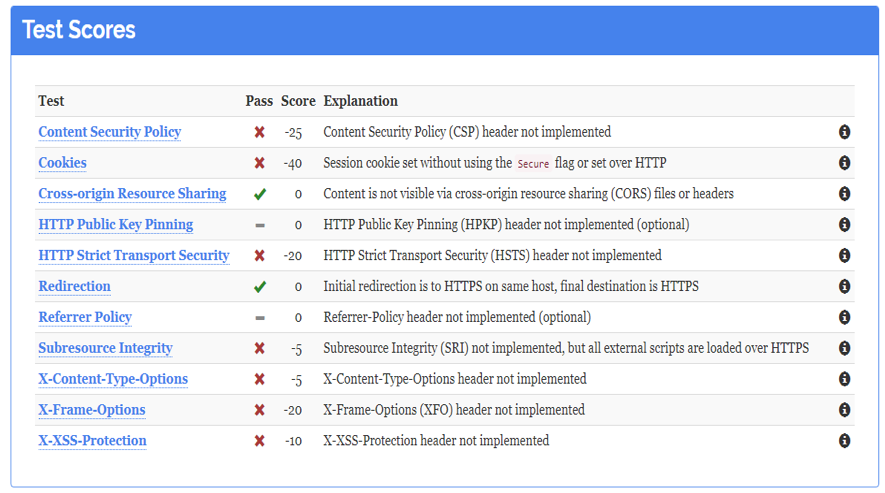
\includegraphics[width=0.8\linewidth]{Graphics/eergebnisobser.png}
	\caption[Egebniss vom HTTP Observatory]{ Ergebnis vom HTTP Observatory }
	\label{fig: HTTP Observatory: Ergebnis}
\end{figure}

\textbf{TLS}

Die betrachtenden von uns Webseite verwendet Signaturverfahren SHA-256-With-RSA. Das bedeutet, dass eine Kombination zwischen SHA256 (kryptologi-schen Hashfunktion, die Hashwerte mit einer Länge zwischen 256 und 512 Bits erzeugt) und \ac{RSA} (ermöglicht symmetrische Schlüssel jeder üblichen Länge verschlüsselt zu werden). In der Abbildung \ref{fig: TSL Observatory: Ergebnis} stellt dar

\begin{figure}[h]
	\centering
	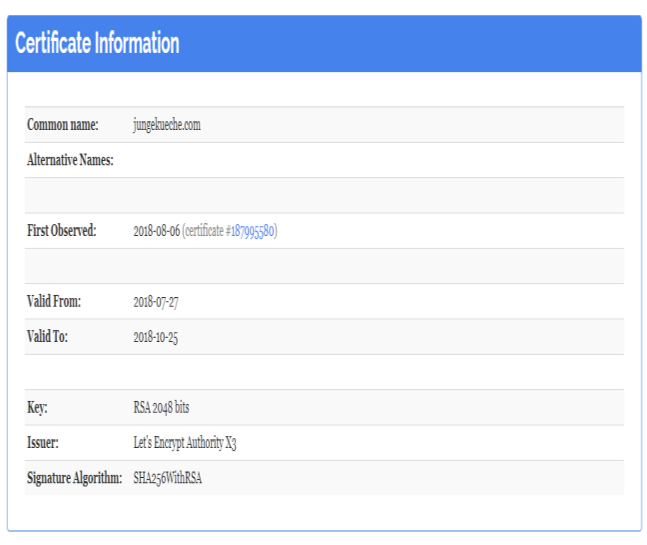
\includegraphics[width=0.8\linewidth]{Graphics/obser2.png}
	\caption[Egebniss TSL Observatory]{Ergebnis vom TLS Observatory}
	\label{fig: TSL Observatory: Ergebnis}
\end{figure}

\section{Warum ist eine Migration notwendig?}

ASP ist eine nicht Objekt-Orientierte Skripte Sprache. Es ist anfällig zu Unter-brechung der Applikationen, z. B. wenn \ac{IIS} gestoppt und neu gestartet wird. Wenn eine ASP-Seite aufgerufen wird, wird den Text linear analysiert.
Die Frontend Verwendung des Bestellsystems ist verschachtelt und es gibt redundanten Optionen. Auf einer Seite befindet sich Login- und Registrierung Menü, sowie das Bestellformular. Das verlangsamt die Eröffnung der Seite. 
Es gibt unnötige Quellcode, das entfernt werden kann. Ein anderer Nachteil des Systems ist, dass es nicht dynamisch orientiert ist, d.h. die Umgebung ist nicht Benutzerfreundlich. Der Auftragsgeber muss sich für jede nötige Änderung bei dem Entwickler melden. Das macht den Benutzer abhängig von dem Hersteller des Programms.
Heutzutage gibt es vielfältige Auswahl von CMS, durch das der Auftragsgeber mit verbreiteten Möglichkeiten zu Änderun-gen seiner Website verfügt. 
Im folgenden Kapitel wird einer diesen CMS erläutert.




